\documentclass{article}
\usepackage{amsmath}
\usepackage[margin=1.5cm]{geometry}
\usepackage{graphicx}
\begin{document}

\begin{center}
	{\huge \textbf{Part 3: Geometry}}

	Calculators are allowed in this section
\end{center}

\bigskip

\section{Area of Rectangles}

\bigskip

\textbf{Calculate the area. If necessary, round to the nearest tenth}

\bigskip

\begin{figure}[!htb]
	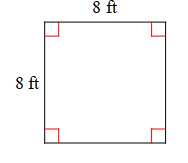
\includegraphics[width=0.3\linewidth]{RectangleArea2.png}
	\qquad\qquad
	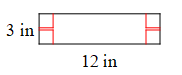
\includegraphics[width=0.3\linewidth]{RectangleArea3.png}
\end{figure}

\section{Area of Parallelograms}

\bigskip

\textbf{Calculate the area. If necessary, round to the nearest tenth}

\bigskip

\begin{figure}[!htb]
	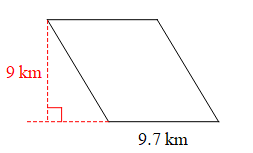
\includegraphics[width=0.3\linewidth]{ParallelogramArea1.png}
	\qquad\qquad
	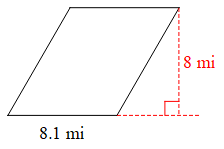
\includegraphics[width=0.3\linewidth]{ParallelogramArea3.png}
\end{figure}


\section{Area of Kites}

\bigskip

\textbf{Calculate the area. If necessary, round to the nearest tenth}

\bigskip

\begin{figure}[!htb]
	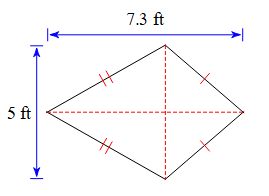
\includegraphics[width=0.3\linewidth]{KiteArea1.png}
	\qquad\qquad
	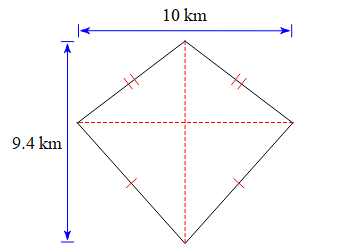
\includegraphics[width=0.3\linewidth]{KiteArea2.png}
\end{figure}

\bigskip

\section{Area of Trapezoids}

\bigskip

\textbf{Calculate the area. If necessary, round to the nearest tenth}

\begin{figure}[!htb]
	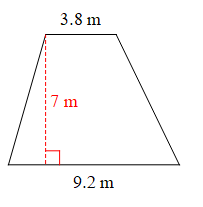
\includegraphics[width=0.3\linewidth]{TrapezoidArea1.png}
	\qquad\qquad
	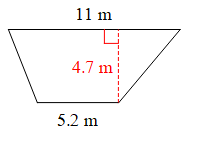
\includegraphics[width=0.3\linewidth]{TrapezoidArea2.png}
\end{figure}

\bigskip

\section{Area of Triangles}

\bigskip

\textbf{Calculate the area. If necessary, round to the nearest tenth}

\begin{figure}[!htb]
	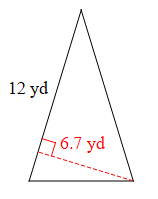
\includegraphics[width=0.16\linewidth]{TriangleArea1.png}
	\qquad
	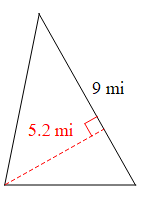
\includegraphics[width=0.16\linewidth]{TriangleArea2.png}
	\qquad
	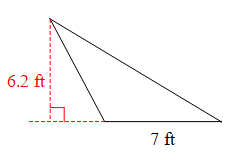
\includegraphics[width=0.25\linewidth]{TriangleArea3.png}
	\qquad
	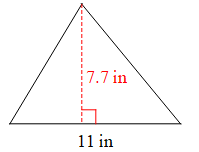
\includegraphics[width=0.25\linewidth]{TriangleArea4.png}
\end{figure}

\bigskip

\section{Area of Circles}

\bigskip

\textbf{Calculate the area. Leave $\pi$ in your answer or round to the nearest tenth}

\bigskip

\begin{figure}[!htb]
	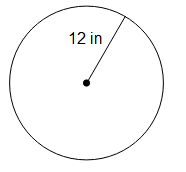
\includegraphics[width=0.2\linewidth]{CircleArea1.png}
	\qquad
	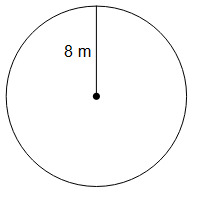
\includegraphics[width=0.2\linewidth]{CircleArea2.png}
\end{figure}

\bigskip

\section{Circumference}

\bigskip

\textbf{Calculate the circumference. Leave $\pi$ in your answer or round to the nearest tenth}

\bigskip

\begin{figure}[!htb]
	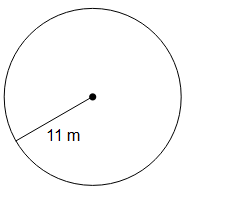
\includegraphics[width=0.16\linewidth]{Circumference1.png}
	\qquad\qquad
	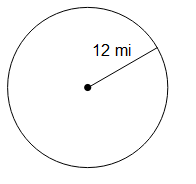
\includegraphics[width=0.16\linewidth]{Circumference2.png}
\end{figure}

\section{Area of Sectors}

\bigskip

\textbf{Calculate the area. Leave $\pi$ in your answer or round to the nearest tenth}

\bigskip

\begin{figure}[!htb]
	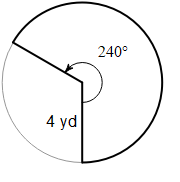
\includegraphics[width=0.16\linewidth]{Sector1.png}
	\qquad\qquad
	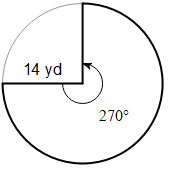
\includegraphics[width=0.16\linewidth]{Sector2.png}
	\qquad\qquad	
	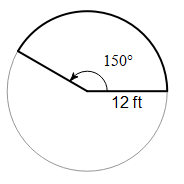
\includegraphics[width=0.16\linewidth]{Sector3.png}
	\qquad\qquad
	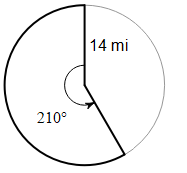
\includegraphics[width=0.16\linewidth]{Sector4.png}
\end{figure}

\section{Volume of Rectangular Prisms}

\bigskip

\textbf{Calculate the volume. If necessary, round to the nearest tenth}

\bigskip

\begin{figure}[!htb]
	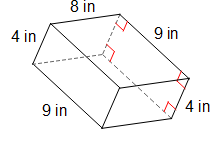
\includegraphics[width=0.2\linewidth]{PrismVolume1.png}
	\qquad\qquad
	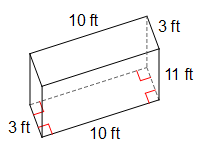
\includegraphics[width=0.2\linewidth]{PrismVolume2.png}
\end{figure}

\section{Volume of Spheres}

\bigskip

\textbf{Calculate the volume. Leave $\pi$ in your answer or round to the nearest tenth}

\bigskip

\begin{figure}[!htb]
	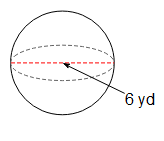
\includegraphics[width=0.16\linewidth]{SphereVolume1.png}
	\qquad\qquad
	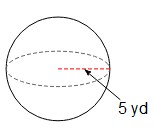
\includegraphics[width=0.16\linewidth]{SphereVolume2.png}
\end{figure}

\bigskip

\section{Volume of Cylinders}

\bigskip

\textbf{Calculate the volume. Leave $\pi$ in your answer or round to the nearest tenth}

\begin{figure}[!htb]
	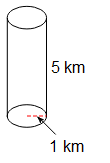
\includegraphics[width=0.16\linewidth]{CylinderVolume1.png}
	\qquad
	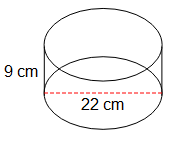
\includegraphics[width=0.16\linewidth]{CylinderVolume2.png}
	\qquad	
	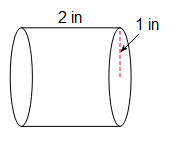
\includegraphics[width=0.16\linewidth]{CylinderVolume3.png}
	\qquad
	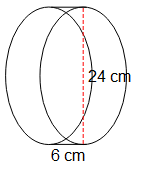
\includegraphics[width=0.16\linewidth]{CylinderVolume4.png}
\end{figure}

\bigskip

\section{Volume of Pyramids}

\bigskip

\textbf{Calculate the volume. If necessary, round to the nearest tenth}

\bigskip

\begin{figure}[!htb]
	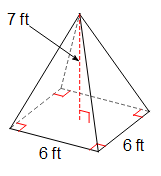
\includegraphics[width=0.2\linewidth]{PyramidVolume2.png}
	\qquad\qquad	
	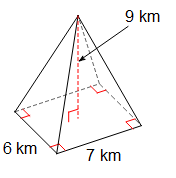
\includegraphics[width=0.2\linewidth]{PyramidVolume3.png}
	\qquad\qquad
	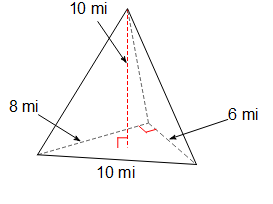
\includegraphics[width=0.3\linewidth]{PyramidVolume4.png}
\end{figure}

\section{Volume of Cones}

\bigskip

\textbf{Calculate the volume. If necessary, round to the nearest tenth}

\bigskip


\begin{figure}[!htb]
	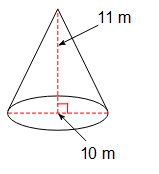
\includegraphics[width=0.2\linewidth]{ConeVolume1.png}
	\qquad\qquad
	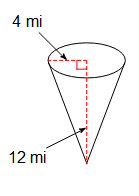
\includegraphics[width=0.2\linewidth]{ConeVolume2.png}
\end{figure}


\section{Surface Area of Solids}

\bigskip

\textbf{Calculate the surface area. If necessary, round to the nearest tenth}

\bigskip

\begin{figure}[!htb]
	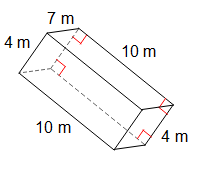
\includegraphics[width=0.18\linewidth]{SA1.png}
	\qquad
	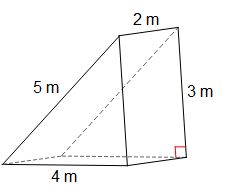
\includegraphics[width=0.18\linewidth]{SA2.png}
	\qquad
	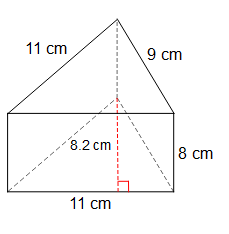
\includegraphics[width=0.18\linewidth]{SA3.png}
	\qquad
	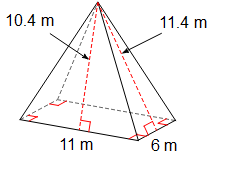
\includegraphics[width=0.18\linewidth]{SA4.png}
\end{figure}

\begin{figure}[!htb]
	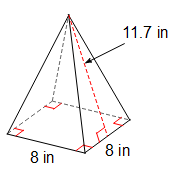
\includegraphics[width=0.18\linewidth]{SA5.png}
	\qquad
	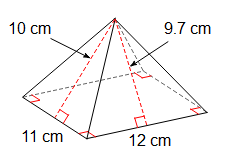
\includegraphics[width=0.18\linewidth]{SA6.png}
	\qquad
	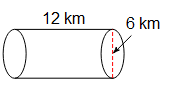
\includegraphics[width=0.18\linewidth]{SA7.png}
	\qquad
	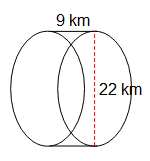
\includegraphics[width=0.18\linewidth]{SA8.png}
\end{figure}

\section{Surface Area of Spheres}

\bigskip

\textbf{Calculate the surface area. If necessary, round to the nearest tenth}
\bigskip
\begin{figure}[!htb]
	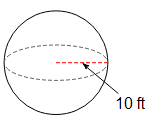
\includegraphics[width=0.2\linewidth]{SASphere1.png}
	\qquad\qquad
	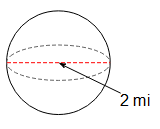
\includegraphics[width=0.2\linewidth]{SASphere2.png}
\end{figure}

\bigskip


\section{Arc Length}

\bigskip

\textbf{Find the length of each arc. Leave $\pi$ in your answer or round to the nearest tenth}

\bigskip

\begin{figure}[!htb]
	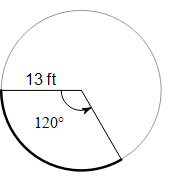
\includegraphics[width=0.16\linewidth]{ArcLength1.png}
	\qquad\qquad
	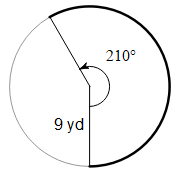
\includegraphics[width=0.16\linewidth]{ArcLength2.png}
	\qquad\qquad
	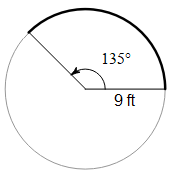
\includegraphics[width=0.16\linewidth]{ArcLength3.png}
	\qquad\qquad
	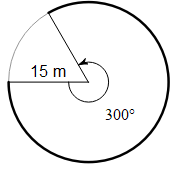
\includegraphics[width=0.16\linewidth]{ArcLength4.png}
\end{figure}

\bigskip

\section{Angle Relationships}

\bigskip

\textbf{Calculate the measure of angle b}

\bigskip


\begin{figure}[!htb]
	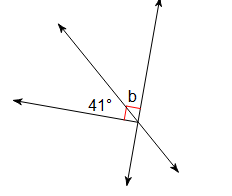
\includegraphics[width=0.15\linewidth]{Complementary1.png}
	\qquad
	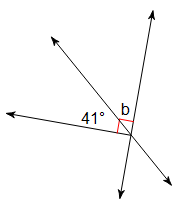
\includegraphics[width=0.15\linewidth]{Complementary2.png}
	\qquad
	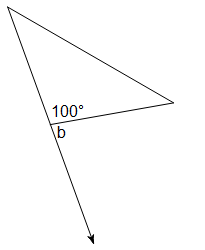
\includegraphics[width=0.15\linewidth]{Sup1.png}
	\qquad
	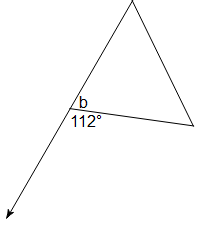
\includegraphics[width=0.15\linewidth]{Sup2.png}
	\qquad
	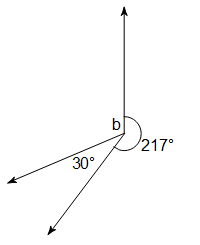
\includegraphics[width=0.15\linewidth]{Angle1.png}
\end{figure}

\begin{figure}[!htb]
	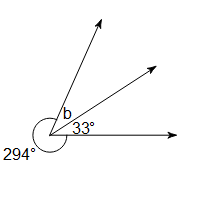
\includegraphics[width=0.15\linewidth]{Angle2.png}
	\qquad
	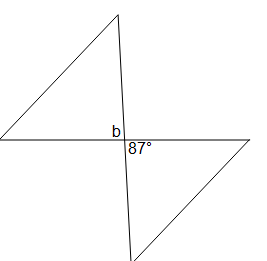
\includegraphics[width=0.15\linewidth]{Ver1.png}
	\qquad
	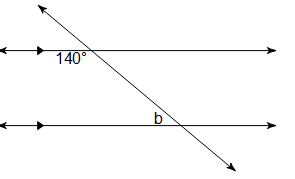
\includegraphics[width=0.15\linewidth]{Angle3.png}
	\qquad
	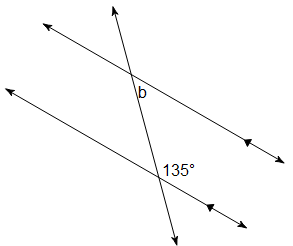
\includegraphics[width=0.15\linewidth]{Angle4.png}
	\qquad
	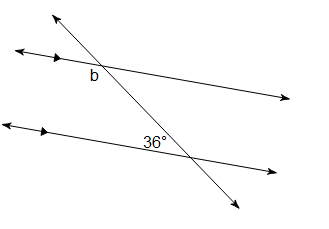
\includegraphics[width=0.15\linewidth]{Angle6.png}
\end{figure}

\begin{figure}[!htb]
	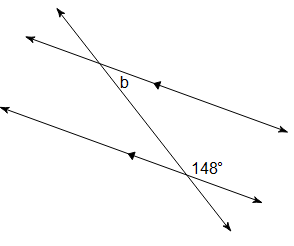
\includegraphics[width=0.15\linewidth]{Angle8.png}
	\qquad
	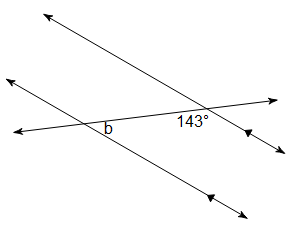
\includegraphics[width=0.15\linewidth]{Angle9.png}
	\qquad
	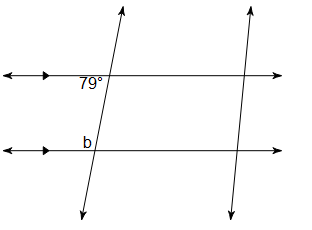
\includegraphics[width=0.15\linewidth]{Angle10.png}
	\qquad
	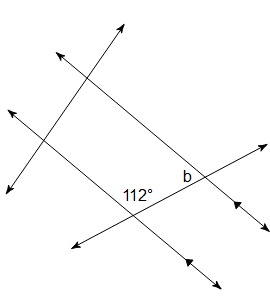
\includegraphics[width=0.15\linewidth]{Angle11.png}
	\qquad
	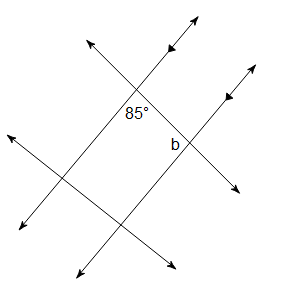
\includegraphics[width=0.15\linewidth]{Angle12.png}
\end{figure}

\begin{figure}[!htb]
	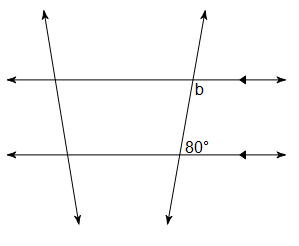
\includegraphics[width=0.15\linewidth]{Angle13.png}
	\qquad
	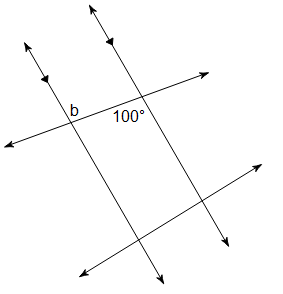
\includegraphics[width=0.15\linewidth]{Angle14.png}
	\qquad
	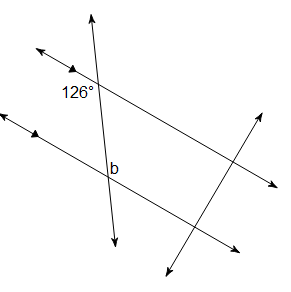
\includegraphics[width=0.15\linewidth]{Angle15.png}
	\qquad
	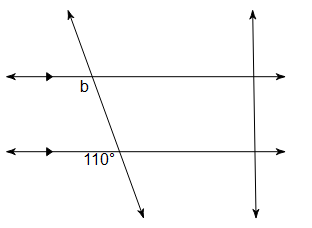
\includegraphics[width=0.15\linewidth]{Angle16.png}
	\qquad
	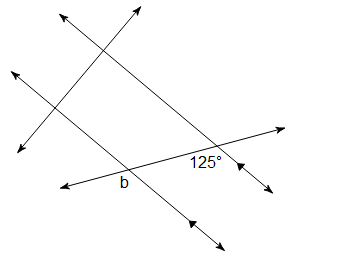
\includegraphics[width=0.15\linewidth]{Angle17.png}
\end{figure}

\bigskip

\section{Pythagorean Thereom}

\bigskip

\textbf{Find the missing side length. Leave radicals in answer (simplify if you can)}

\bigskip

\begin{figure}[!htb]
	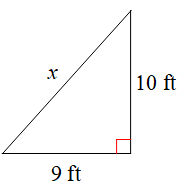
\includegraphics[width=0.15\linewidth]{Pyth1.png}
	\qquad\qquad
	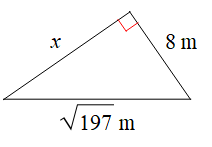
\includegraphics[width=0.15\linewidth]{Pyth2.png}
	\qquad\qquad
	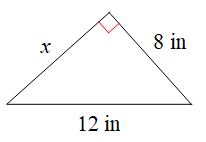
\includegraphics[width=0.15\linewidth]{Pyth3.png}
	\qquad\qquad
	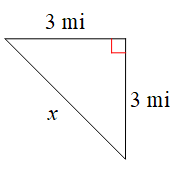
\includegraphics[width=0.15\linewidth]{Pyth4.png}
\end{figure}


\newpage
\bigskip

\section{Converse Pythagorean Thereom}

\bigskip

\textbf{State whether the triangle is acute, obtuse, or right}

\bigskip



\begin{figure}[!htb]
	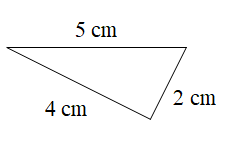
\includegraphics[width=0.15\linewidth]{Con1.png}
	\qquad\qquad
	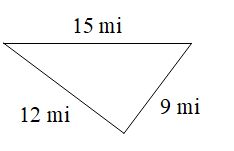
\includegraphics[width=0.15\linewidth]{Con2.png}
	\qquad\qquad
	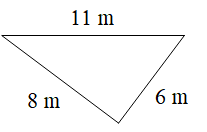
\includegraphics[width=0.15\linewidth]{Con3.png}
	\qquad\qquad
	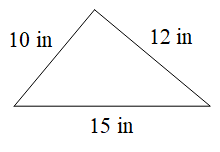
\includegraphics[width=0.15\linewidth]{Con4.png}
\end{figure}

\bigskip

\section{Transformations}

\bigskip

\textbf{Graph the given transformation}

\bigskip

	\text{Translation: 2 units left and 4 units down}\qquad\qquad\qquad\qquad 
	\text{Translation: 4 units left}
\begin{figure}[!htb]
	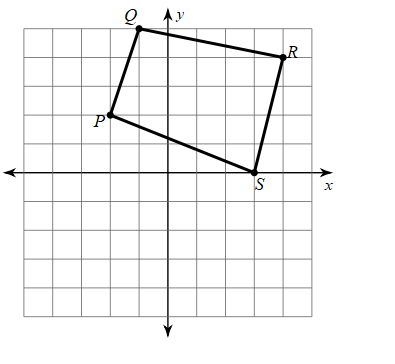
\includegraphics[width=0.4\linewidth]{Trans1.png}
	\qquad\qquad
	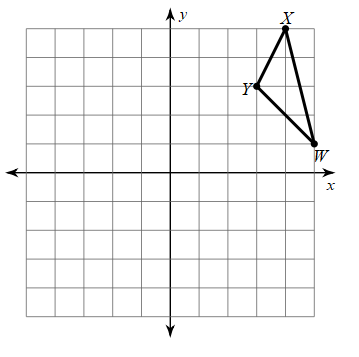
\includegraphics[width=0.38\linewidth]{Trans2.png}
\end{figure}

\bigskip

	\text{Rotation 90\textdegree counterclockwise about the origin}\qquad\qquad\qquad 
	\text{Rotation 180\textdegree about the origin}
\begin{figure}[!htb]
	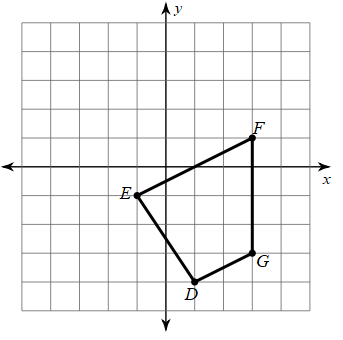
\includegraphics[width=0.35\linewidth]{Trans3.png}
	\qquad\qquad\qquad
	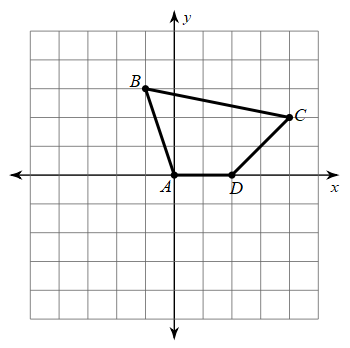
\includegraphics[width=0.37\linewidth]{Trans4.png}
\end{figure}

\newpage

\bigskip

	\text{Reflection across the x-axis}\qquad\qquad\qquad\qquad\qquad\qquad\qquad
	\text{Reflection across the y-axis}
\begin{figure}[!htb]
	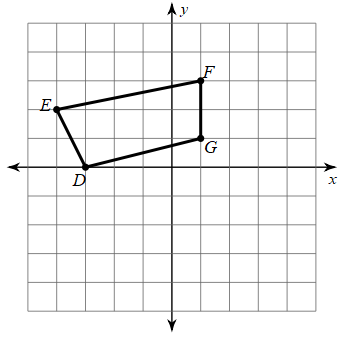
\includegraphics[width=0.4\linewidth]{Trans5.png}
	\qquad\qquad
	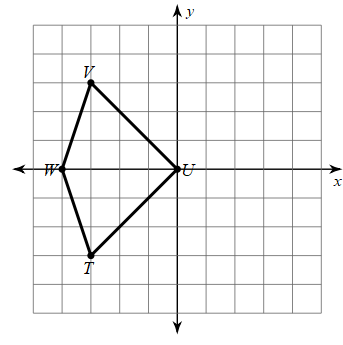
\includegraphics[width=0.4\linewidth]{Trans6.png}
\end{figure}

\bigskip

	\text{Dilation of $\frac{3}{2}$ about the origin}\qquad\qquad\qquad\qquad\qquad\qquad\qquad 
	\text{Dilation of 2 about the origin}
\begin{figure}[!htb]
	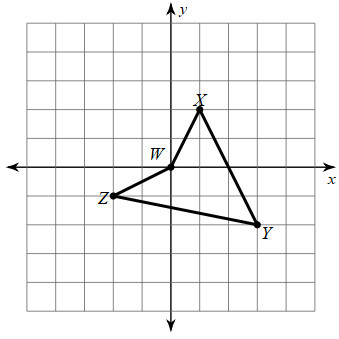
\includegraphics[width=0.4\linewidth]{Trans7.png}
	\qquad\qquad
	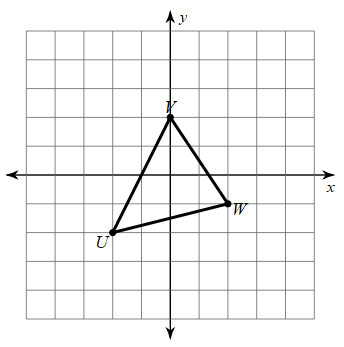
\includegraphics[width=0.4\linewidth]{Trans8.png}
\end{figure}

\end{document}
